
Il mio compito nello sviluppo dell'applicazione è stato quello 
di creare un prototipo iniziale avendo a disposizione un mock up creato con
proto.io\cite{protoio} e una serie di requisiti essenziali.

\section{Requisiti essenziali}

La base di partenza di QIX sono state delle funzionalità essenziali e 
sonstanzialmente molto difficili da inserire in una versione dell'app già avanzata.
È stati quindi deciso di creare un prototipo di partenza avente i seguenti requisiti:

\begin{itemize}
    \item {
        \textbf{Navigazione dinamica}: L'applicazione deve gestire dei cambiamenti di contesto
        dinamici: dev'essere possibile mostrare all'utente contenuti dinamici indipendentemente
        dal contesto in cui si trova.
    }
    \item {
        \textbf{QIX Shake}: Tale funzionalità dell'applicazione
        deve essere disponibile in una qualunque sezione o vista si trovi l'utente
        e la sua funzione deve essere determinata dal contesto attuale;
    } 
    \item {
        \textbf{Animazioni interattive}: L'intera applicazione dev'essere progettata in modo tale da presentare all'utente
        delle \textbf{animazioni interattive} in stile CardView\cite{cardview} disponibili in 
        qualunque sezione o vista in cui si trovi l'utente e definite dal contesto attuale;

        Le animazioni in questione devono essere progettate in pagine, in cui ogni pagina può contenere 
        più CardView. L'utente vedrà in un determinato momento una e soltanto una pagina.

        Ogni CardView deve essere trascinabile dall'utente e deve interagire con le altre CardView della pagine. 
        Quando l'utente usa una forza di trascinamento superiore a un valore di soglia tutte le viste devono
        cadere per gravità;
        
        Tale gravità finirà con la fine dell'animazione o l'apparizione di una nuova pagina se presente;
    }
    \item {
        \textbf{Autenticazione}: L'applicazione deve supportare tre diversi stati o modalità di autenticazione:
        \begin{enumerate}
            \item\textbf{Trial Mode}: l'utente è anonimo, esiste solo un id per tenere traccia dei suoi QIX coins.
            \item\textbf{Signed Mode}: l'utente ha inserito il numero di telefono e il suo genere;
            \item \textbf{Pro Mode}: l'utente aggiunge dei dati su se stesso o collega il suo account a dei social media come Facebook, Google o Instagram;
        \end{enumerate}
        Si nota facilmente che non esiste una stato in cui l'utente non è registrato: questo perchè
        per tenere traccia dei suoi QIX coins e di altri dati utili è necessario avere una riferimento all'utente;
    }
    \item {
        \textbf{DeepLinks}: L'applicazione deve poter essere avviata dinamicamente
        attraverso dei \textbf{Deep Links}\cite{deeplinks};
        E deve essere in grado di gestirli in base al contesto dell'utente;
    }
\end{itemize}

\section{La navigazione dinamica}

% Analizzando il requisito mi sono posto diverse domande: \\ \\
% \noindent{
%     \large\textit{Cosa significa dinamicamente?}
%     \normalsize{Il nostro obiettivo in questo caso è mostrare all'utente \textbf{contenuti diversi}
%     indipendentemente dal constesto e quindi dalla vista in cui si trova}\\ \\
%     \large\textit{Quale contesto?}
%     \normalsize{Con contesto dell'utente si intende lo stato attuale dell'applicazione,
%     quindi l'intero stack di navigazione se presente;
%     } \\ \\
% }

Prima di entrare nel merito della soluzione al problema, spiego brevemente gli
standard di navigazione delle app iOS.

Ogni applicazione può avere degli \textbf{UINavigationController}\cite{navigationcontroller},
ossia dei contenitori di \textbf{UIViewController}\cite{viewcontroller} che vengono
utilizzati per mantenere lo stack di navigazione e gestire la transizioni tra due UIViewController.

Nella figura~\ref{fig:1} si nota facilmente come il Navigation controller gestisce un'array di View Controller e una sola 
navigation bar

% Ogni \textbf{UIViewController}\cite{viewcontroller} 
% può avere un \textbf{UINavigationController}\cite{navigationcontroller}, ossia un costrutto che contiene una barra di navigazione superiore 
% e una serie di APIs per mostrare nuovi UIViewController
Esistono tre tipologie base di navigazione:

\begin{figure}
    \centering
    \begin{minipage}[b]{0.4\textwidth}
        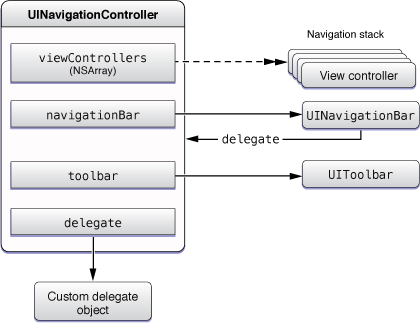
\includegraphics[width=\textwidth]{navigation}
        \caption{Navigation controller scheme}
        \label{fig:1}
    \end{minipage}
    %   \hfill
    %   \begin{minipage}[b]{0.4\textwidth}
    %     
\includegraphics[width=\textwidth]{logo}
    %     \caption{Picture 2}
    %     \label{fig:2}
    %   \end{minipage}
\end{figure}

\begin{enumerate}
    \item{\textbf{Push}: un UIViewController avente un navigation controller può rendere
    visibile un altro ViewController attraverso la funzione
    \begin{center}
        \begin{tabular}{c}
        \begin{lstlisting}
func pushViewController(_ viewController: UIViewController, animated: Bool)
        \end{lstlisting}
        \end{tabular}
    \end{center}
    di un Navigation controller
    }
    \item{\textbf{Modal}: un ViewController può presentare un altro ViewController senza necessariamente avere un 
    Navigation Controller
    }
\end{enumerate}


\normalsize